\documentclass{standalone}
\usepackage{amsmath}
\usepackage[compat=1.1.0]{tikz-feynman}

\definecolor{MyBlue}{RGB}{0, 68, 136}
\definecolor{MyYellow}{RGB}{221, 170, 51}
\newcommand{\lw}{0.8pt}

\begin{document}
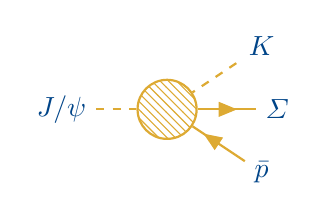
\begin{tikzpicture}[every edge/.append style={line width=\lw}]
  \begin{feynman}
    \vertex[text=MyBlue] (jpsi)  at (-1.34, 0.0) {$J/\psi$};
    \vertex[text=MyBlue] (ks)    at ( 1.2,  0.8) {$K$};
    \vertex[text=MyBlue] (sigma) at ( 1.4,  0.0) {$\varSigma$};
    \vertex[text=MyBlue] (pbar)  at ( 1.2, -0.8) {$\bar{p}$};
    \vertex[blob, draw=MyYellow, line width=\lw, pattern color=MyYellow] (B) at (0,0) {};
    \diagram*{
    (jpsi) -- [scalar, color=MyYellow] (B),
    (B)    -- [anti fermion, color=MyYellow] (pbar),
    (B)    -- [fermion, color=MyYellow] (sigma),
    (B)    -- [scalar, color=MyYellow, dash phase=2pt] (ks),
    };
  \end{feynman}
\end{tikzpicture}
\end{document}
